\documentclass{amsart}

% \usepackage[notref,notcite]{showkeys}
\usepackage[style=authoryear,ibidtracker=false,uniquename=false,giveninits=true,terseinits=true,maxbibnames=5,backend=biber]{biblatex}
\usepackage{float}
\usepackage{graphicx}
\usepackage{todonotes}
\usepackage{subcaption}


\renewbibmacro{in:}{}
\addbibresource{rnni_polynomial.bib}

\newtheorem{lemma}{Lemma}
\newtheorem{theorem}{Theorem}

\newcommand{\rnni}{\mathrm{RNNI}}
\newcommand{\findpath}{\textsc{FindPath}}
\newcommand{\mrca}{\mathrm{mrca}}
\newcommand{\rank}{\mathrm{rank}}
\newcommand{\nni}{\mathrm{NNI}}

\graphicspath{{figures/}}

\begin{document}


\begin{lemma}
    Let $p = \findpath(T,R)$ be the path from tree $T$ to $R$ that is computed by the $\findpath$ algorithm.
    Let $\hat{T}$ be the tree at the beginning of iteration $i$ of the algorithm in which the most recent common ancestor of cluster $C_i$ is moved down.
    Then there is no tree on $p$ where a cluster $C_j$ of $R$ with $\rank((C_i)_{\hat{T}}) \geq \rank((C_j)_{\hat{T}})$ and $i < j$ has the same most recent common ancestor as $C_i$.
\end{lemma}

\proof

For proving the lemma by contradiction we assume that clusters $C_i, C_j$ exist such that their most recent common ancestors do not coincide in $\hat{T}$, but in some tree following this one on $p$.
Let $T''$ be the first tree where the most recent common ancestors coincide and let $T'$ be the tree on $p$ that is immediately followed by $T''$.
It is obvious that the $\rnni$ between $T'$ and $T''$ is an $\nni$ move.
It is $\rank((C_i)_{T'}) = \rank((C_j)_{T'}) + 1$ and $\rank((C_i)_{T''}) = \rank((C_j)_{T''}) = \rank((C_j)_{T'})$.
Considering the illustration in Figure~\ref{fig:nni_move}, we can follow from the second equality that $C_i, C_j \subseteq A \cup C$, which is contradicting $\rank((C_i)_{T'}) = \rank((C_j)_{T'}) + 1$, as this implies $C_j \cap B \neq \emptyset$ in that figure.


\begin{figure}[H]
\centering
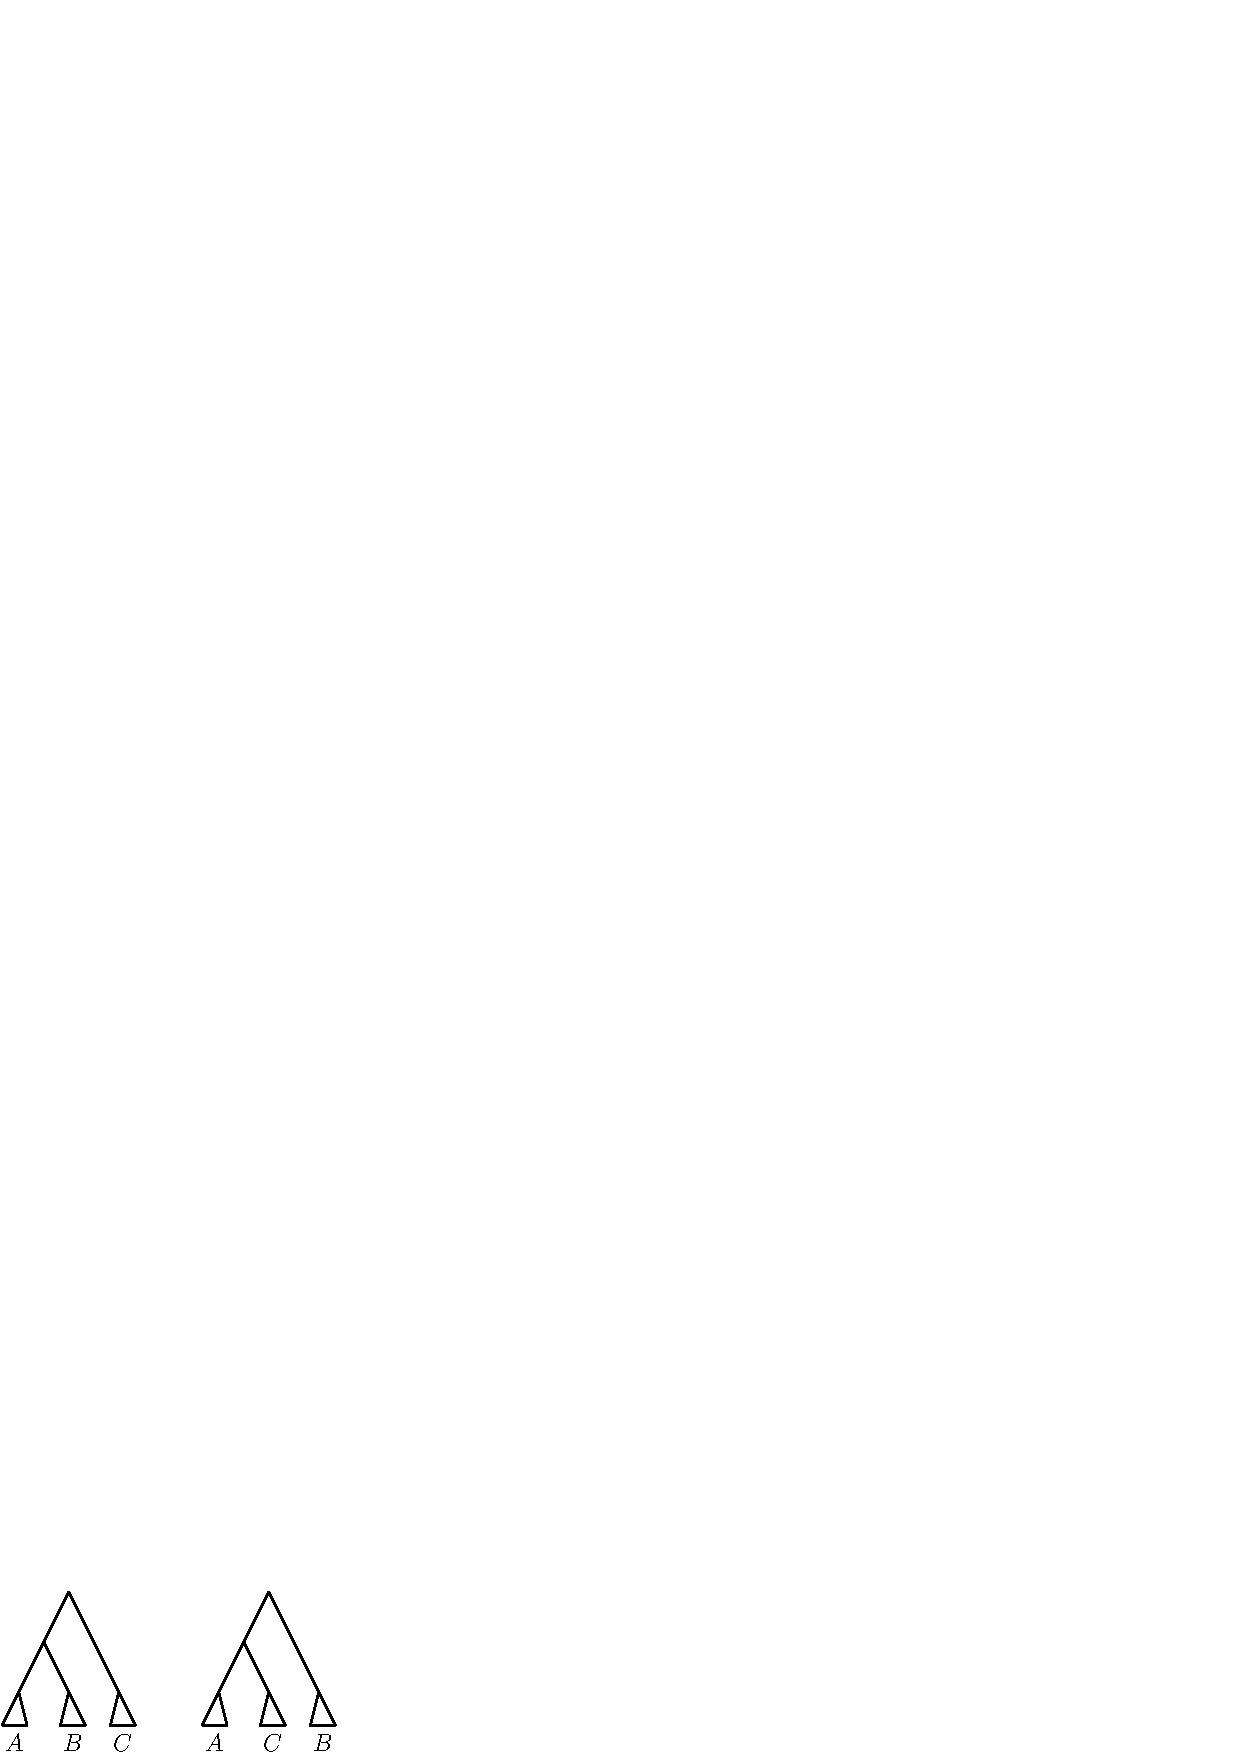
\includegraphics[width=0.4\textwidth]{NNI_move}
\vspace{12pt}
\caption{$\nni$ move}
\label{fig:nni_move}
\end{figure}

\endproof

\begin{lemma}
    Let $T$ and $R$ be ranked trees.
    If for all neighbours $T' \in N_1(T)$ of $T$ it is $d_{FP}(T',R) \geq d_{FP}(T,R) - 1$, then it is $d_{\rnni}(T,R) = d_{FP}(T,R)$.
\end{lemma}

\proof
    We prove this lemma by induction on the distance $d_{\rnni}(T,R)$.
    It is easy to see that the statement is true for the base case $d_{\rnni}(T,R) = 1$.
    Let us consider trees $T$ and $R$ with distance $d_{\rnni}(T,R) = d+1$ and assume that the lemma is true for all pairs of trees with distance less than $d+1$.
    For contradiction we assume that $d_{FP}(T,R) > d_{\rnni}(T,R) = d+1$.
    There must be a tree $T'' \in N_1(T)$ that has $\rnni$ distance $d_{\rnni}(T'',R) = d$.
    With the induction hypothesis it follows $d_{FP}(T'',R) = d$, which contradicts that it is $d_{FP}(T',R) \geq d_{FP}(T,R) - 1 > d$ for all trees $T' \in N_1(T)$.
    Therefore, it cannot be $d_{FP}(T,R) > d_{\rnni}(T,R)$ which concludes the proof of the lemma.
\endproof


\begin{theorem}
    Let $T,R$ be trees and $p = \findpath(T,R)$ the path from $T$ to $R$ computed by $\findpath$.
    Let $d_{FP}(T,R)$ denote the $\findpath$ distance from $T$ to $R$, that is the length of $p$.
    For all $T' \in N_1(T)$ it is $d_{FP}(T',R) \geq d_{FP}(T,R) - 1$, where $N_1(T)$ is the one-neighbourhood of $T$.
\end{theorem}

\proof
For contradiction we assume that for the pair $T,R$ of trees there is a tree $T' \in T$ with $d_{FP}(T',R) < d_{FP}(T,R) - 1$.
We also assume that $T,R$ is the pair with minimum $\findpath$ distance $d_{FP}(T,R)$ among those trees fulfilling this property.
It immediately follows that the first move on $p = \findpath(T,R)$ changes one of the nodes $v,w$ that bound the interval $[v,w]$ on which the $\rnni$ move between $T$ and $T'$ is performed.
\todo{introduce notion of interval}
This is due to the fact that otherwise the first steps on $p$ and $p' = \findpath(T',R)$ coincide, as $T$ and $T'$ only differ by the interval $[v,w]$, which contradicts the assumption that $T$ and $R$ are the closest pair of trees for which we can find such a $T'$.

In this proof we will at first distinguish the case that there is an $\nni$ move between $T$ and $T'$ from the case that there is a rank swap.
For each of these cases we further distinguish between all moves possible on the tree $T$ on $p$, which happen on the intervals adjacent to $[v,w]$.
Note that $p$ is the path computed by $\findpath$, so there is a cluster $C_k$ whose most recent common ancestor moves down by the $\rnni$ move following $T$ on $p$.
We denote the tree following $T$ on $p$ by $\hat T$.

At first we consider the case that there is an $\nni$ move between $T'$ and $T$ as illustrated in the top of Figure~\ref{fig:thm_fp_nni1}.
It follows that $(v,w)$ is an edge in $T$.
Let us now distinguish different types of moves between $T$ and $\hat T$ on intervals incident to $v$ or $w$.

\begin{enumerate}
    \item $\nni$ move on edge $(v,w)$

    If this $\nni$ move results in $\hat T = T'$, it is $d_{FP}(T',R) = d_{FP}(T,R) - 1$, which contradicts the assumption on the choice of $T'$.
    Otherwise $\hat T$ follows $T'$ on $p'$ as well, meaning that the remaining part of $p$ and $p'$ coincide, and it follows $d_{FP}(T',R) = d_{FP}(T,R)$.
    This is true as $(C_k)_T$ that is moved down by $\findpath$ on this move must contain taxa in one of the subtrees below $v$ and in the subtree below $w$ that does not contain $v$, for example $B$ and $C$ in Figure~\ref{fig:thm_fp_nni1}.
    And as $(C_k)_T'$ moves down on $p'$ as well, the move made on $T'$ is an $\nni$ move that results in the same tree as the one following $T$ on $p$.
    This is again a contradiction to the assumption $d_{FP}(T',R) < d_{FP}(T,R) - 1$.

    \begin{figure}[!hbt]
    \centering
    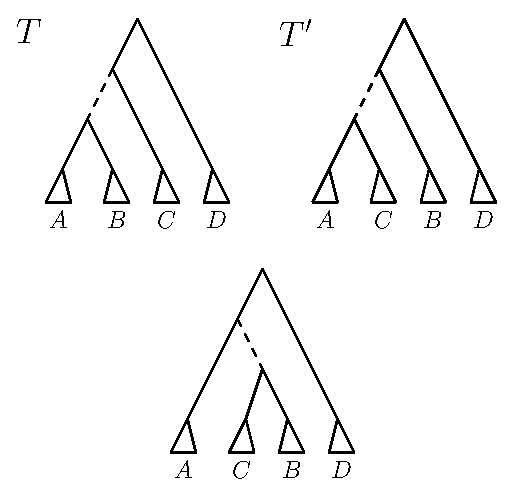
\includegraphics[width=0.4\textwidth]{thm_fp_nni1}
    \vspace{12pt}
    \caption{$\nni$ move between $T$ and $T'$ on the dashed edge $(v,w)$ and the third $\rnni$ neighbour resulting from a move on that edge.}
    \label{fig:thm_fp_nni1}
    \end{figure}

    \item $\nni$ moves on edge $(u,v)$ above $(v,w)$

    Notice that this is only possible if the interval above $(v,w)$ is an edge.
    As it is depicted in the top of Figure~\ref{fig:thm_fp_nni2a}, there are two $\nni$ moves on $(u,v)$ possible that lead to different trees.
    We denote the subtrees that are children of $w$ by $A$ and $B$, the one of $v$ not containing $w$ by $C$ and the one of $u$ not containing $v$ by $D$, according to the labels in Figure~\ref{fig:thm_fp_nni2a}.
    \todo{We call both cluster and subtrees $A,B,C$ and $D$}

    \begin{figure}[H]
        \begin{subfigure}[b]{.45\textwidth}
            \centering
            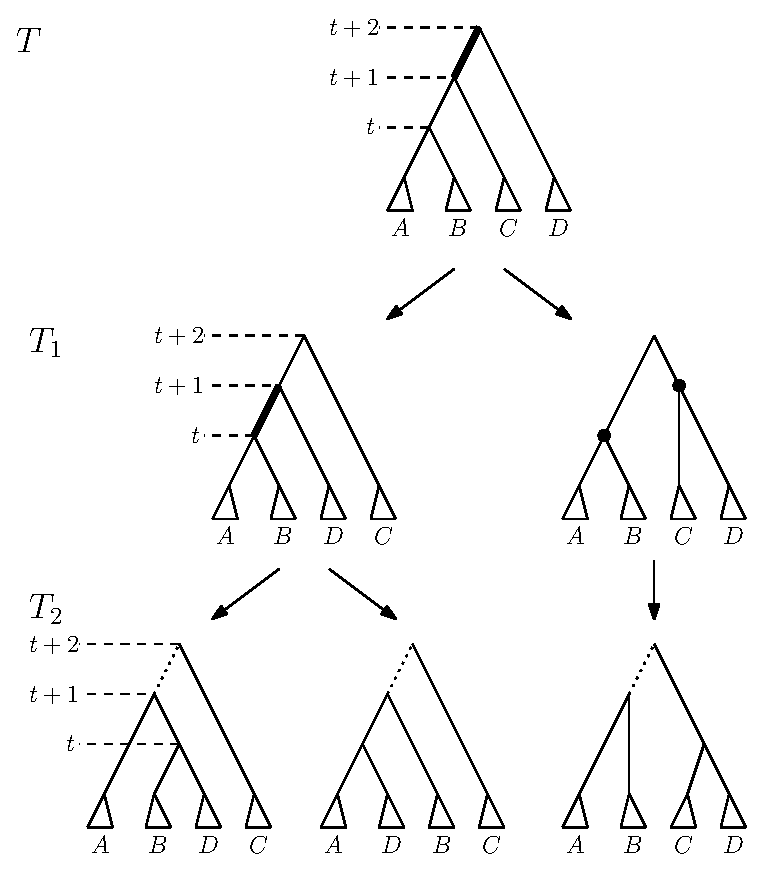
\includegraphics[width=0.9\linewidth]{thm_fp_nni2a.eps}
            \vspace{12pt}
            \caption{path $p$ following $T$}
            \label{fig:thm_fp_nni2a}
        \end{subfigure}
        \begin{subfigure}[b]{.45\textwidth}
            \centering
            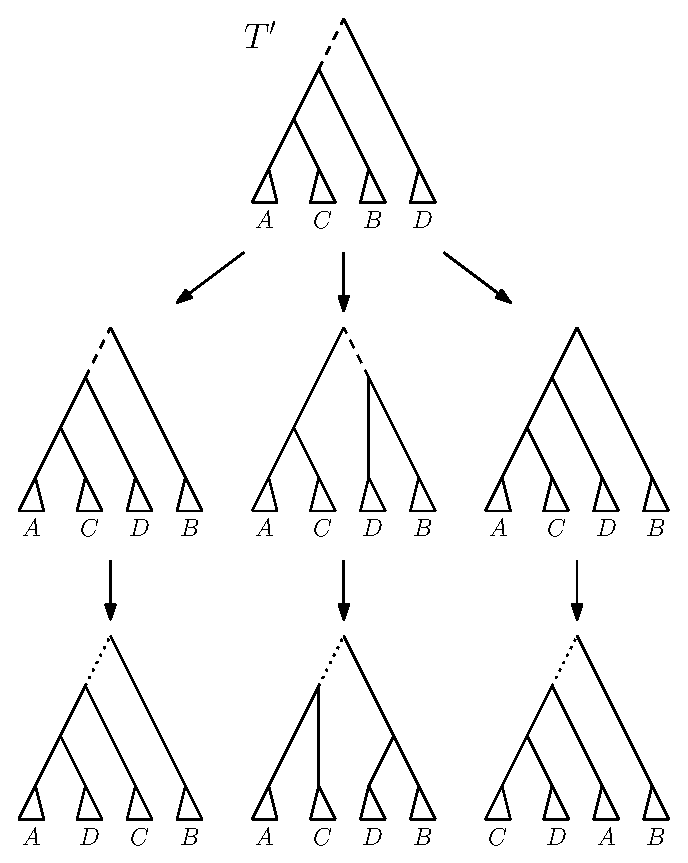
\includegraphics[width=0.9\linewidth]{thm_fp_nni2b.eps}
            \vspace{12pt}
            \caption{path $p'$ following $T'$}
            \label{fig:thm_fp_nni2b}
        \end{subfigure}
        \caption{Comparison of $p$ and $p'$ if there is an $\nni$ move on the edge $f$ above $e$ in $T$.
        The trees on the bottom are those following $T$ and $T'$ on $p$ and $p'$ after two $\rnni$ moves, respectively, depending on the cluster $C_k$ that is currently considered on $\findpath$:
        ${C_k \subseteq A \cup D}$ on the left, ${C_k \subseteq B \cup D}$ in the middle, ${C_k \subseteq C \cup D}$ on the right.}
    \end{figure}

    All moves on edge $(u,v)$ of $T$ that could happen on $p$ are depicted in Figure~\ref{fig:thm_fp_nni2a}.
    We will now consider each of these moves separately.
    If $\hat T$ is the tree at the top left of Figure~\ref{fig:thm_fp_nni2a}, which results from $T$ by exchanging the subtrees $C$ and $D$, the cluster $C_k$ that is moved down by $\findpath$ is either a subset of $A \cup B \cup D$, $A \cup D$ or $B \cup D$.

    \begin{enumerate}
        \item
            If $C_k \subseteq A \cup B \cup D$, then $C_k$ reached it's final position in $\hat T$ on $p$.
            Specifically, the subtree containing $A \cup B$ in $T$ is the same subtree in $R$, by the nature of $\findpath$.
            It follows that on $p'$ there is a move that moves the most recent common ancestor of $A \cup B$ down right before $C_k$ is considered.
            This means that the tree following $T'$ on $p'$ is $T$, contradicting $d_{FP}(T',R) < d_{FP}(T,R) - 1$.
        \item
            If $C_k \subseteq A \cup D$, the move on $\hat T$ on $p$ moves $(C_k)_{\hat T}$ further down by exchanging $B$ and $D$, resulting in the tree in the bottom left of Figure~\ref{fig:thm_fp_nni2a}.
            As the same most recent common ancestor $(C_k)_{T'} \subseteq A \cup D$ moves down on $p'$, the two moves following $T'$ move the subtree $D$ down by exchanging it with its neighbours $B$ and $C$ as depicted on the left of Figure~\ref{fig:thm_fp_nni2b}.
            Comparing the trees on $p$ and $p'$ after the two moves following $T$ and $T'$, respectively, shows that we are again at a stage where two trees on these paths only differ by one edge (dotted edges in the trees at the bottom left of Figures~\ref{fig:thm_fp_nni2a} and~\ref{fig:thm_fp_nni2b}).
            Furthermore, the relation of the distancesof these tree to $R$ are the same as the ones from $T$ and $T'$ to $R$, which contradicts the assumption that $T$ and $R$ are the closest pair of trees with this relation.
        \item
            If $C_k \subseteq B \cup D$, the two $\rnni$ moves following $T$ and $T'$ on $p$ and $p'$, respectively, end up in the trees depicted in the tree in the middle at the bottom of Figures~\ref{fig:thm_fp_nni2a} and \ref{fig:thm_fp_nni2b}, analogous to the previous case.
            As in the previous case, these trees coincide in all but one interval (dotted edges in the figure), which again contradicts the assumptions on $T$ and $R$.
    \end{enumerate}

    If the $\nni$ move on $(u,v)$ results in a tree $\hat T$ containing a subtree $C \cup D$ as illustrated on the top right of Figure~\ref{fig:thm_fp_nni2a}, it is $C_k \subseteq C \cup D$.
    If $(C_k)_T$ does not move further down on $p$, it follows that $A \cup B$ is a cluster in $R$ and that before $C_k$ is considered on $p'$, $(A \cup B)_{T'}$ moves down by one $\rnni$ move.
    This means that $T$ follows $T'$ on $p'$, which contradicts $d_{FP}(T',R) < d_{FP}(T,R) - 1$.
    If on the other side the rank of $(C_k)_T$ decreases further on $p$, the move on $\hat T$ is a rank swap as depicted in the bottom right of Figure~\ref{fig:thm_fp_nni2a}.
    The moves on $p'$ that decreases the rank of $(C_k)_{T'}$ are $\nni$ moves exchanging $D$ with $B$ and $A$, because it is $C_k \subseteq C \cup D$.
    These moves are shown on the right of Figure~\ref{fig:thm_fp_nni2b}.
    As above, the two trees resulting from the two moves following $T$ and $T'$ on $p$ and $p'$, respectively, coincide by all but one interval.
    Therefore, we end up in the same contradiction as above.

    \item Rank move on interval $[u,v]$ above $(v,w)$

    Notice that this is only possible if $[u,v]$ is a rank interval.
    If after the rank move, which increases the rank of $v$, there is a rank move on $\hat T$ that increases the rank of $w$, the same rank moves happen on $p'$ and the trees after these two moves on $p$ and $p'$ coincide in all but one interval.
    As previously, this contradicts the assumption that $T$ and $R$ are the closest trees where there is a $T' in N_1(T)$ with $d_{FP}(T',R) < d_{FP}(T,R) - 1$.
    If on the other side there is no such rank move on $\hat T$, then the cluster induced by $w$ is a cluster in $R$ as well.
    The tree following $T'$ on $p'$ is $T$ as it is the result of building this cluster in $T'$, which happens right before the cluster $C_k$ is being considered on $p'$.
    This is due to the order in which $\findpath$ considers most recent common ancestors of clusters.
    This contradicts $d_{FP}(T',R) < d_{FP}(T,R) - 1$.

    \item $\rnni$ moves on interval below $[v,w]$

    If there is a move on the interval below $[v,w]$, $C_k$ is a subset of $A \cup B$, following the notions of the trees in the top of Figure~\ref{fig:thm_fp_nni1}.
    In this case, the move following $T'$ on $p'$ exchanges $B$ and $C$ by an $\nni$ move first, which moves $(C_k)_{T'}$ down and transforms $T'$ into $T$, contradicting $d_{FP}(T',R) < d_{FP}(T,R) - 1$.
\end{enumerate}

Let us now assume that there is a rank move between $T$ and $T'$ where nodes $v$ and $w$ inducing clusters $A$ and $B$ swap ranks as depicted in Figure~\ref{fig:thm_fp_rank1}.
We will again consider the different moves from $T$ to $\hat T$ that are possible on intervals adjacent to $(v,w)$, which is the interval of the rank move between $T$ and $T'$.


\begin{figure}[!hbt]
\centering
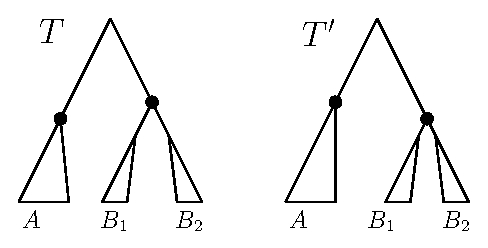
\includegraphics[width=0.4\textwidth]{thm_fp_rank1}
\vspace{12pt}
\caption{Rank move between $T$ and $T'$ on the interval given by the highlighted nodes}
\label{fig:thm_fp_rank1}
\end{figure}

\begin{enumerate}
    \item Rank move on $[v,w]$

    The only possible move on $(v,w)$ on $T$ is a rank move resulting in $\hat T = T'$.
    It follows $d_{FP}(T',R) = d_{FP}(T,R) - 1$, which obviously contradicts our assumption $d_{FP}(T',R) < d_{FP}(T,R) - 1$.

    \item $\nni$ move on edge above $[v,w]$

    Notice that this is only possible if the interval above $[v,w]$ is an edge $(u,v)$.
    In this case the $\nni$ move builds a new cluster containing taxa of $B$ and of the subtree $C$ that is the child of $u$ that does not contain $v$, as depicted in the top left of Figure~\ref{fig:thm_fp_rank2}.
    It follows that $C_k \subseteq C \cup B_1$ where $B_1$ is one of the subtrees that is child of $w$.
    If there was rank move following on $\hat T$ decreasing the rank of $(C_k)_{\hat T}$, it follows that the node inducing cluster $A$ has the same rank in $T$ as in $R$.
    In this case the tree following $T'$ on $p'$ must be $T$ as $(A)_{T'}$ moves to it's final position on $\findpath$ before $C_k$ is moved down.
    However, this contradicts $d_{FP}(T',R) < d_{FP}(T,R) - 1$.
    Let us now consider what happens if there is a rank move on $\hat T$ that decreases the rank of $(C_k)_{\hat T}$ on $p$.
    This case is depicted on the left of Figure~\ref{fig:thm_fp_rank2}.
    The moves happening on $p'$ are as follows.
    First the rank of $(C_k)_{T'}$ decreases by a rank swap of $(C \cup B)_{T'}$ and $(A)_{T'}$ on $T'$ and then an $\nni$ move exchanges $B_2$ and $C$, as it is depicted on the right of the same figure.
    One can easily see that the two trees on $p$ and $p'$ that are two $\rnni$ moves apart from $T$ and $T'$, respectively, only differ by one interval.
    Again, this is a contradiction to the fact that $T$ and $R$ are the trees with minimum distance for which we can find a $T' \in N_1(T)$ with $d_{FP}(T',R) < d_{FP}(T,R) - 1$.

    \begin{figure}[!hbt]
    \centering
    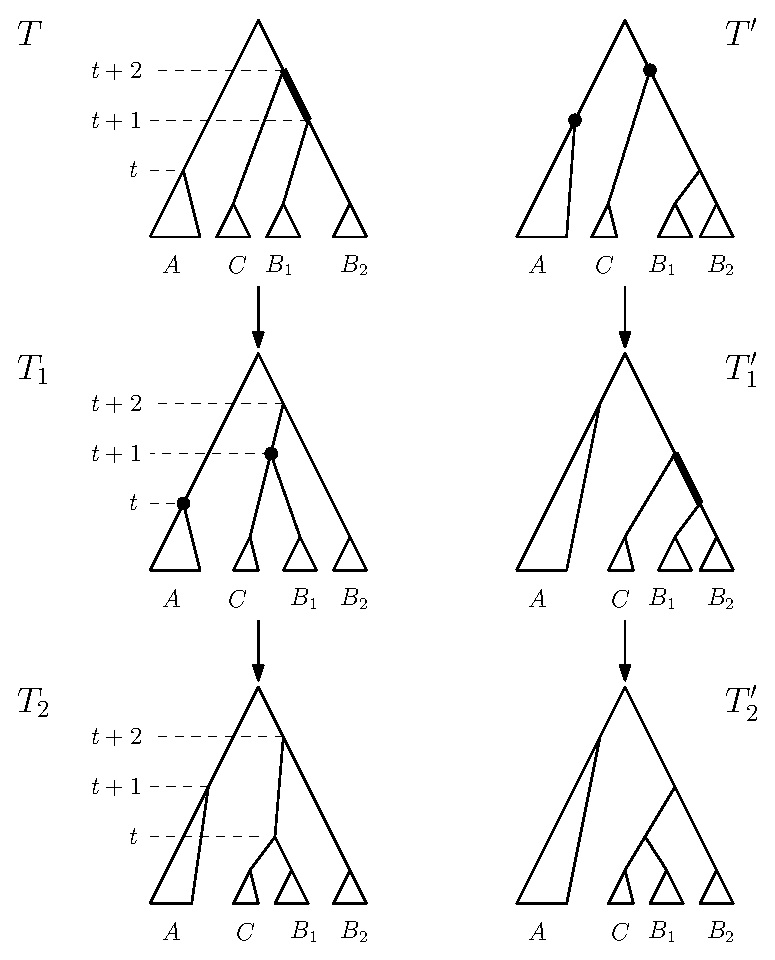
\includegraphics[width=0.4\textwidth]{thm_fp_rank2}
    \vspace{12pt}
    \caption{Comparison of $p$ (left) and $p'$ (right) if there is a rank move between $T$ and $T'$ and an $\nni$ move on the edge below the corresponding rank interval follows on $p$.}
    \label{fig:thm_fp_rank2}
    \end{figure}

    \item Rank move on interval above $[v,w]$

    Notice that this is only possible if the interval above $[v,w]$ is a rank interval.
    If there is a rank move increasing the rank of $v$, and no rank move increasing the rank of $w$ immediately afterwards, $C_k$ reaches it's final position in the tree $\hat T$ on $p$ following $T$.
    It follows that the cluster $A$ induced by $w$ in $T$ is a cluster in $R$ as well.
    This means that the move following $T'$ on $p'$ leads to $T$, as the node inducing $A$ moves down before $C_k$ is considered on $\findpath$.
    This contradicts $d_{FP}(T',R) < d_{FP}(T,R) - 1$.
    If on the other side the rank swap on $T$ is directly followed by a rank swap increasing the rank of $w$, the same moves happen on $p'$ and the trees following $T$ and $T'$ after two $\rnni$ moves on $p$ and $p'$, respectively, coincide in all but one interval.
    And this again is a contradiction to our choice of $T$ and $R$.

    \item $\rnni$ moves on interval below $[v,w]$

    If there is a move on the interval below $[v,w]$, it follows that $\findpath$ moves $C_k \subseteq A$ down where $A$ is the cluster induced by $w$.
    For decreasing the rank of the most recent common ancestor of $C_k \subseteq A$ in $T'$, the move on $T'$ must be a rank swap that results in $T$, contradicting  $d_{FP}(T',R) < d_{FP}(T,R) - 1$.
\end{enumerate}

We can conclude that in any of the above cases we end up in a contradiction, proving that a tree $T'$ with $d_{FP}(T',R) < d_{FP}(T,R) - 1$ does not exist in $N_1(T)$.
Therefore we can follow that $d_{FP}(T',R) \geq d_{FP}(T,R) -1$ for all $T' \in N_1(T)$.
\endproof

\begin{lemma}
Let $T$ and $R$ be $\rnni$ trees such that $\findpath(T, R)$ terminates after two iterations and returns a path $p$ of length $\ell$.
Then $\ell = d(T, R)$.
\end{lemma}

\proof
Case 1: $R = [\{1, 2\}, \{3, 4\}, \ldots]$.

Let $T'$ be the running tree after the first iteration of $\findpath(T, R)$.
Define
\[
s(T, R) = (\rank(\{1,2\})_T - 1) + (\rank(\{3,4\})_{T'} - 2)
\]
where $\rank(S)_T$ is the rank of the most recent common ancestor of cluster $S$ in tree $T$.
Note that an inductive argument implies that it is enough to show that $s(T_1, R) \geq s(T, R) - 1$ for all $T_1 \in N_1(T)$.
This means that there is no tree $T_1 \in N_1(T)$ that is more than one $\rnni$ move closer to $R$ than $T$.

For the following it is important to notice that the following holds for the path $p$ computed by $\findpath(T,R)$.
If $\mrca_T(\{1,2\}) > \mrca_T(\{3,4\})$, then there is no tree on $p$ where $\mrca(\{1,2\}) = \mrca(\{3,4\})$.

If this was possible on $p$, it could only result from an $\nni$ move that moves $\mrca(\{1,2\})$ down, and not from a rank swap.
An $\nni$ move that moves $\mrca(\{1,2\})$ down exchanges two subtrees, one of them containing taxon $1$ or $2$, the other one none of the two.
Let us call these are the subtrees $B$ and $C$ of Figure~\ref{fig:nni_move}, and without loss of generality assume that $1 \in A$ and $2 \in B$.
If after this move it is $\mrca(\{1,2\}) = \mrca(\{3,4\})$, then one of the taxa $3,4$ is in $A$ and the other one in $C$.
But then it must have been $\mrca(\{1,2\}) = \mrca(\{3,4\})$ in the tree just before this $\nni$ move already.
Therefore, it cannot be $\mrca(\{1,2\}) = \mrca(\{3,4\})$ on a tree on $p$, if it is $\mrca_T(\{1,2\}) \neq \mrca_T(\{3,4\})$ in the start tree $T$.

So let now $T_1 \in N_1(T)$ and let $T''$ be the tree after the first iteration of $\findpath(T_1,R)$. We will distinguish different possible $\rnni$ moves between $T$ and $T_1$ and consider how the path $\findpath(T_1,R)$ changes compared to $\findpath(T,R)$.

\begin{enumerate}

    \item The $\rnni$ move between $T$ and $T_1$ does not change the rank of $\mrca(\{1,2\})$ or $\mrca(\{3,4\})$

    It is obvious that $\rank(\{1,2\})_{T_1} = \rank(\{1,2\})_{T}$ as well as $\rank(\{3,4\})_{T''} = \rank(\{3,4\})_{T'}$, as the move between $T$ and $T_1$ does not have an effect of the ranks of these most recent common ancestors in $T$ or $T'$.
    Therefore, it is $s(T, R) = s(T_1,R)$.

    \item The $\rnni$ move between $T$ and $T_1$ changes $\rank(\mrca(\{1,2\}))$, which is not equal to $\rank(\mrca(\{3,4\}))$

    If this $\rnni$ move increases the rank of $\mrca(\{1,2\})$, the first move on $\findpath(T_1,R)$ will decrease the rank of this most recent common ancestor and results in the tree $T$, which gives us $\rank(\{1,2\})_{T_1} = \rank(\{1,2\})_{T} - 1$.
    If otherwise the rank of $\mrca(\{1,2\})$ decreases by the $\rnni$ move from $T$ to $T_1$, it is $\rank(\{1,2\})_{T_1} = \rank(\{1,2\})_T - 1$.
    However, the rank of $\mrca(\{3,4\})$ is the same in $T'$ and $T''$, no matter whether $\rank(\mrca(\{1,2\}))$ decreases or increases.
    The only point at which $\rank(\mrca(\{3,4\}))$ could change on the path is if there is an exchange of ranks of $\mrca(\{1,2\})$ and $\mrca(\{3,4\})$ in the first iteration of $\findpath(T_1,R)$.
    But this just happens if and only if the same exchange of ranks happens on $\findpath(T,R)$, hence it is $s(T_1,R) \geq s(T,R) - 1$ in this case.

    \item The $\rnni$ move between $T$ and $T_1$ changes $\rank(\mrca(\{1,2\}))$, which is equal to $\rank(\mrca(\{3,4\}))$

    If the move from $T$ to $T_1$ increases the rank of $\mrca(\{1,2\})$, the first tree on $\findpath(T_1,R)$ is $T$, as there always is exactly one $\rnni$ move that moves $\mrca(\{1,2\})$ down, which in this case is the move that moves both $\mrca(\{1,2\})$ and $\mrca(\{3,4\})$ down.
    Then it is $\rank(\{1,2\})_{T_1} = \rank(\{1,2\})_{T} + 1$ and $\rank(\{3,4\})_{T''} = \rank(\{3,4\})_{T'}$ and therefore $s(T_1,R) = s(T,R) + 1$ in this case.
    And if the rank of $\mrca(\{1,2\})$ decreases from $T$ to $T_1$, $T_1$ is the first tree on $\findpath(T,R)$, which results in $s(T_1,R) = s(T,R) - 1$.

    \item The $\rnni$ move between $T$ and $T_1$ changes $\rank(\mrca(\{3,4\}))$, which is not equal to $\rank(\mrca(\{1,2\}))$

    In this case it obviously is $\rank(\{1,2\})_{T_1} = \rank(\{1,2\})_{T}$.
    Also, the rank of $\mrca(\{3,4\})$ changes on the path from $T_1$ to $T''$ if and only if it does on the path from $T$ to $T'$.
    Note that this rank can change by at most one when this most recent common ancestor exchanges ranks with $\mrca(\{1,2\})$.
    Therefore, it is either $\rank(\{3,4\})_{T''} = \rank(\{3,4\})_{T'} + 1$ or $\rank(\{3,4\})_{T''} = \rank(\{3,4\})_{T'} - 1$, depending on whether the move between $T$ and $T_1$ increases or decreases the rank of $\mrca(\{3,4\})$.
    In either case it is $s(T_1,R) \geq s(T,R) - 1$
\end{enumerate}

We can conclude that in any case it is $s(T_1,R) \geq s(T,R) - 1$.


Case 2: $R = [\{1, 2\}, \{1, 2, 3\}, \ldots]$.

The same as case 1, the only difference is that $\mrca(\{1,2\}) > \mrca(\{1,2,3\})$ is not possible.
%TODO Check whether this really is true!
\endproof
\end{document}
